\chapter{Les machines électriques - Généralités}
\section{Introduction}
	\subsection{Classification des machines électriques}
	Tout se base sur l'interaction des courants électriques et des champs 
	magnétiques. On classes ces bèbètes en trois catégories :
	
	\begin{enumerate}
	\item \textit{Les machines génératrices.} Elles se basent 
	sur l'induction d'un courant électrique dans un circuit conducteur par
	\textbf{déplacement relatif} de celui-ci et d'un champ magnétique. La 
	dynamo (circuit qui tourne dans un champ fixe) et l'alternateur (champ qui tourne dans un circuit fixe) sont de ce type.
	\item \textit{Les moteurs électriques.} Ils sont basés sur 
	l'obtention d'un effort mécanique par l'action d'un champ magnétique sur un circuit traversé par un 
	courant extérieur (pouvant donner lieux à un champ magnétique). Nous 
	pouvons parler ici du moteur à courant continu ou alternatif. L'alternatif peut être de type \textit{synchrone} ou \textit{asynchrone}. 
	\item \textit{Les machines transformatrices.} Leur rôle est 
	de modifier la grandeur des courants et tensions alternatifs par l'induction d'un courant dans un conducteur à l'aide d'un champ magnétique variable dans le temps mais fixe dans l'espace. 
	Le transformateur est le grand classique.
	\end{enumerate}
	
	\subsection{Intérêt des moteurs électriques}
	Ceux-ci ont pas mal d'avantages sur les moteurs thermiques : moins 
	polluants, moins bruyants, démarrent seuls, facilité d'emploi, régularité 
	du couple utile, possibilité de l'inversion du sens de rotation, 
	fort couple vitesse à faible vitesse et même à l'arrêt, \dots Le 
	dernier point est très important car cela les affranchis, par 
	exemple, de boîte à vitesses. En effet, les moteurs thermiques ne 
	disposent pas de cette jouissante propriété et possèdent tout un 
	dispositif mécanique à engrenages, dissipant de l'énergie.
	
	\subsection{Le moteur asynchrone}
	C'est \textbf{le} moteur le plus utilisé. Il fonctionne directement 
	en tension alternative. Celle-ci génère un courant circulant dans le 
	\textbf{stator} constituant la seule source externe de champ mag
	nétique, le 
	rotor n'a pas à être relié à une source d'énergie. Cependant, il existe 
	des courants rotoriques mais ceux-ci sont \textbf{induits} : on parle 
	parfois de \textbf{moteur d'induction}. Ce moteur équipe la quasi 
	totalité des machines-outils classique (tours, fraiseuses, \dots).
	On l'utilise lorsqu'on se soucie peu de la constance de la vitesse et qu'on ne fait
	 pas varier celle-ci dans de larges proportions. Lorsqu'on charge le moteur, la
	 vitesse varie un peu mais ceci est négligeable. Le démarrage se fait
	 directement	  
	 pour les unités de petite puissance. Par contre, pour ceux de forte puissance on
	 démarre sous tension réduite pour éviter un \textbf{appel de courant trop
	 élevé}.
	 Gamme des puissances en triphasé : 1 kW à 10 MW. En dessous de 1 kW on
	 reste dans du monophasé. 
	 
	
	\subsection{Le moteur synchrone}
	Afin de les utiliser, il faut d'abord les faire "roter" à leur 
	\textbf{vitesse nominale} avant de les coupler au réseau, nécessitant un 
	moteur auxiliaire. Ceci se fait à l'aide de l'électronique de puissance. En effet, les
	onduleurs à thyristors fournissent des courants triphasés de fréquence variable
	en tenant compte de la vitesse de rotation du rotor (auto-pilotés). La seule
	différence avec le moteur asynchrone 
	se situe dans la conception du rotor. Ce-dernier est constitué 
	d'aimants (ou alimenté en courant continu). Après le démarrage, le 
	moteur tourne en synchronisme avec le champ tournant. Ces moteurs 
	ne dépendent donc que du réseau qui les alimente et sont ainsi 
	utilisés lorsqu'une rotation uniforme est primordiale.\footnote{
	Différence à plus expliciter plz}
	
	
	\subsection{Les moteurs à courant continu}
	Ils sont les champions dans les très faibles puissances (jouets, 
	essuie-glaces\dots). Leur atout majeur est de posséder une 
	remarquable capacité de variation de vitesse. Ceci se fait grâce à la variation de
	la tension d'alimentation ou intervient de nouveau l'électronique de puissance. Ils
	jouent un rôle 
	important dans la traction électrique et sont alors des
	moteurs "série". On utilise également ces moteurs pour les asservissement de vitesse très performants. 
	
	\subsection{Les autres types de machines électriques}
		\textsc{Les moteurs universels}\\
		On les trouve dans les robots ménagers, ventilateurs, \dots  
		C'est le moteur de la vie domestique. Leur vitesse chute 
		rapidement lorsqu'un couple trop important leur est demandé. Usage limité aux puissances inférieures au kW.\\
		
		\textsc{Les moteurs pas à pas}\\
		Utilisés dans les dispositifs à positionnement précis et ont 
		l'avantage d’être très simple à la conception mais nécessairement associé à de l'électronique de puissance. Les autres machines maintenant une position précise via un frein, cette machine à un aimant au rotor venant se placer devant des bobines qui sont alimentées à tour de rôle en courant continu. 
		
	\subsection{Associations moteurs - électronique}
	Les moteurs à faible puissance, ou les synchrones auto-pilotés pour 
	les fortes sont souvent associés à des équipement électroniques. Même l'asynchrone est combiné pour pouvoir profiter d'une vitesse variable. 
	
	
\section{Méthodes d'étude des machines électriques}
	\subsection{Généralités}
	Pour étudier les machines, deux méthodes s'offrent à nous :
	\begin{enumerate}
	\item \textit{La méthode de Kirchhoff}. On écrit les équations des 
	circuits, la conservation de l'énergie et on déduit le reste. Le 
	dispositif décrit par les équations se présente comme une boite noire 
	s'incluant dans une chaîne de régulation. C'est l'optique de l'
	\textbf{automaticien}.
	\item \textit{La méthode de Maxwell}. On part des grandeurs physiques 
	et on calcule le reste. C'est l'optique du \textbf{constructeur}.
	\end{enumerate}
	Si l'on se base sur le critère de l'utilité pratique, en Belgique (activité réduite en construction de grosses machines électriques), il 
	est plus intéressant de choisir la méthode de Kirchhoff. D'un point de 
	vue formation, cette méthode est également plus "simple" (car 
	systématique). La préférence va ainsi pour Kirchhoff, mais n'oublions 
	pas pour autant la seconde !
	
	\subsection{Choix du phénomène physique exploité}
	On peut concevoir des moteurs capacitifs (loi de Coulomb) ou inductif (
	Laplace). Quasi tous les moteurs sont de type inductif car la densité 
	d'énergie potentielle magnétique ($1/2B^2/\mu_0$) est 10,000 fois 
	supérieure à la densité d'énergie potentielle électrique ($1/2\epsilon_0
	E^2$).\\
	Le dispositif magnétique le plus simple est l'électro-aimant dont 
	la force est donnée par $f_{em} = \frac{1}{2} i^2\frac{dL(x)}{dx}$ où i 
	est le courant parcourant le circuit. Les machines électriques sont donc des machines magnétiques. 
	
	
	
\section{Rappel des lois de l'électromagnétisme}
	\subsection{Loi de la force magnétomotrice (f.m.m.)}
	Elle intervient dans le calcul des ampère-tours nécessaires pour 
	magnétiser un circuit magnétique. Sous sa forme locale 
	\begin{equation}
	\rot \vec{H} = \vec{J}_t
	\end{equation}
	où $\vec{H}$ est le champ magnétique local et $\vec{J}_t$ la 
	densité de courant. La forme intégrale est 
	\begin{equation}
	\mathcal{F} = \oint \vec{H}.\vec{dl} = \sum i
	\label{eq:2.2}
	\end{equation}
	où $\mathcal{F}$ est la force électromotrice le long d'un contour 
	fermé embrassant un faisceau de conducteurs parcourus par des 
	courants $i$.
	
	\subsection{Loi de Maxwell}
	Elle exprime la force électromotrice induite dans un \textbf{circuit}. 
	Sous sa forme locale 
	\begin{equation}
	\rot \vec{E} = -\frac{\partial \vec{B}}{\partial t}
	\end{equation}
	Sous sa forme intégrale 
	\begin{equation}
	e = ri = \oint \vec{E}.\vec{dl} = -\frac{d\Phi}{dt}
	\end{equation}
	La f.e.m. induite $e$ fait alors circuler un courant $i$. Un 
	accroissement du flux fait ainsi circuler un courant négatif de la trigonométrie. 		Si le circuit est fixe et l'induction 
	variable on parle de f.e.m. \textbf{induite}. Si le circuit est 
	mobile, on dira \textbf{engendrée}. Dans ce dernier cas, on écrit 
	alors la loi sous la forme
	\begin{equation}
	de = -[\vec{B}\times\vec{v}].\vec{dl}
	\end{equation}
	où $\vec{v}$ est la vitesse relative par rapport à un champ d'induction 
	$\vec{B}$ d'un élément de longueur $\vec{dl}$ du circuit électrique 
	considéré.
	\newpage
	\textsc{Exemple}
	\begin{wrapfigure}[9]{l}{3.5cm}
	\vspace{-5mm}
	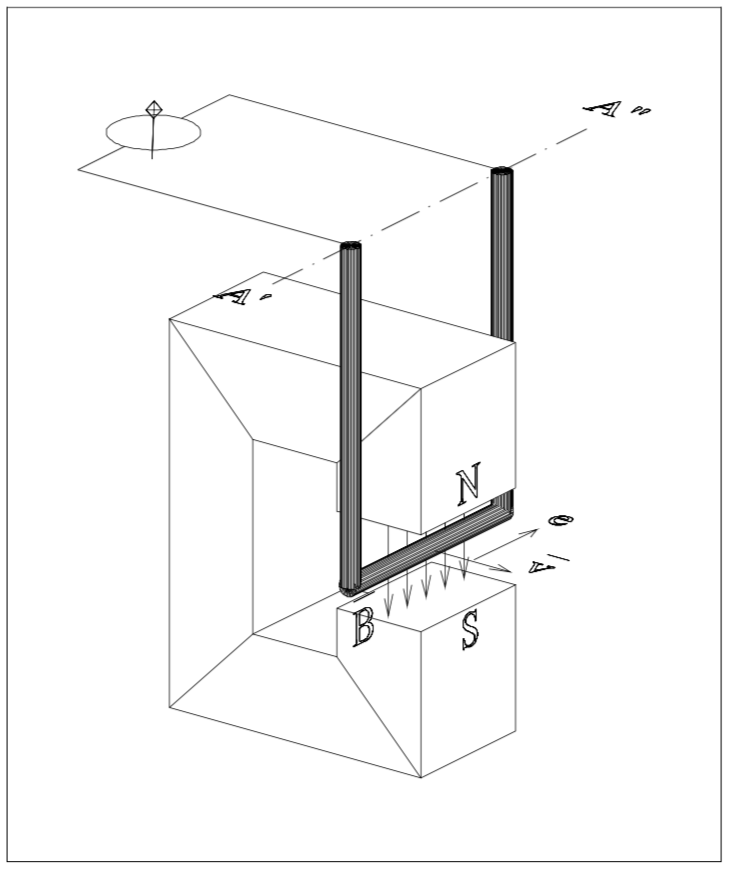
\includegraphics[scale=0.25]{ch2/image1} 
	\captionof{figure}{}
	\end{wrapfigure}
	Soit un conducteur linéaire de longueur $l$ se 
	déplaçant à vitesse constante $\vec{v}$ dans un champ d'induction $\vec{
	B}$ uniforme. Cette loi devient 
	\begin{equation}
	e = -[\vec{B}\times\vec{v}].\vec{l}
	\label{eq:2.6}
	\end{equation}
	Si le déplacement se fait normalement à son axe et à la direction 
	du champ (en valeur absolue) : $e = Blv$.\\
	\textsc{Remarque :} l'existence de la f.m.e induite n'a de sens que lorsque $l$ fait partie d'un \textbf{circuit}.	\\
	
	\subsection{Loi de Laplace}
	Elle donne l'expression de la force sur un conducteur parcouru par 
	un courant plongé dans un champ d'induction $\vec{B}$ par la formule 
	\begin{equation}
		d\vec{F} = -[\vec{B}\times i\vec{dl}]
	\end{equation}
	
	
\section{Principes de fonctionnement des machines électriques}
	\subsection{Éléments constitutifs des machines électriques}
	Quasi toutes contiennent un organe fixe dénommé \textbf{stator} 
	et un organe mobile, le \textbf{rotor}, séparés par un entrefer. 
	L'\textbf{inducteur} est l'organe destiné à créer le flux 
	magnétique, par des aimants permanents ou par des courants 
	électriques. Alors que l'organe siège des forces électromotrices est appelé l'\textbf{induit}. 
	
	
	\subsection{Machines hétéropolaires}
		\subsubsection{Principes de fonctionnement}
		\begin{wrapfigure}[8]{r}{6.5cm}
		\vspace{-5mm}
		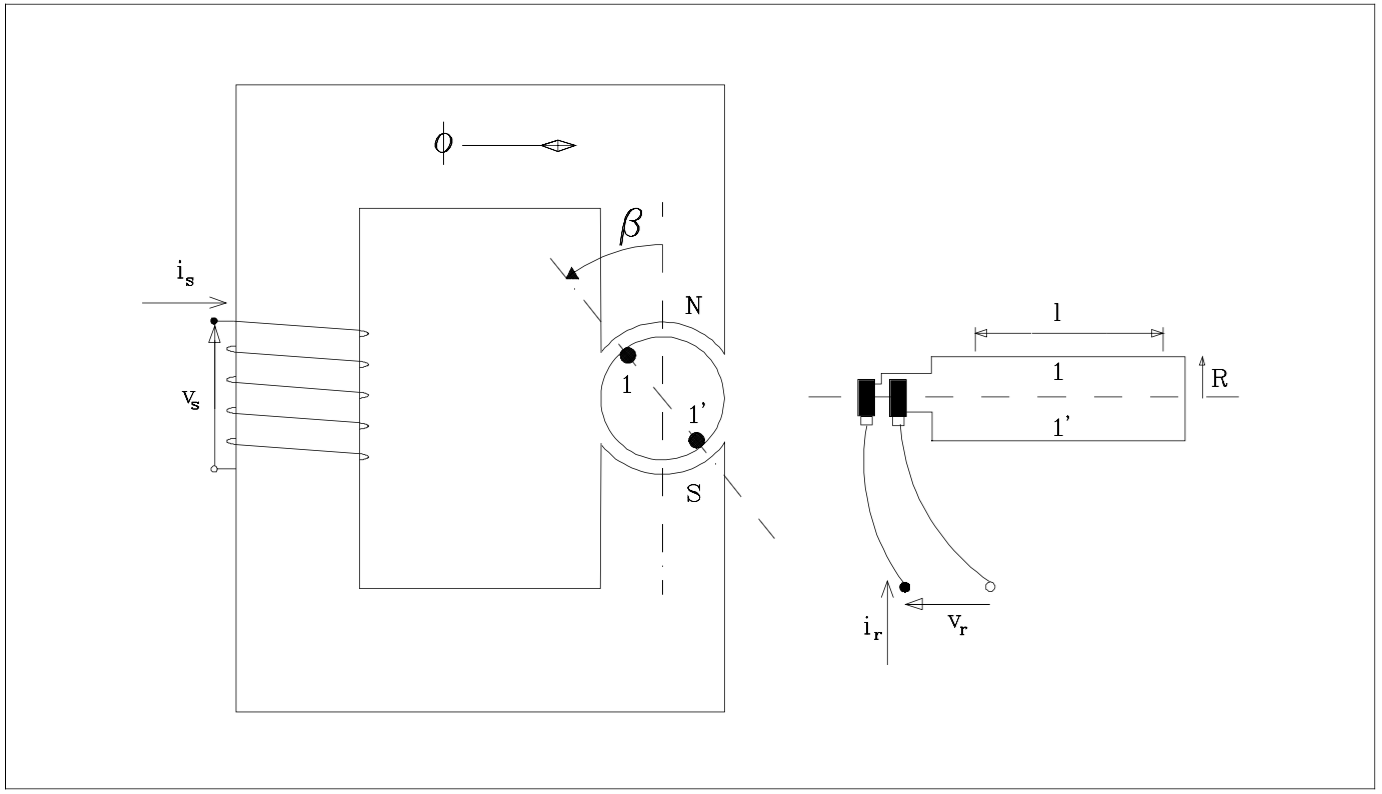
\includegraphics[scale=0.25]{ch2/image2} 
			\captionof{figure}{}
		\end{wrapfigure}
		Hétéropolaire signifie que $\vec{B}$ n'a pas le même signe 
		partout dans l'entrefer. Considérons le dispositif suivant, 
		constitué d'un stator métallique portant un circuit inducteur 
		de $N_S$ spires parcourues par un courant continu $i_s$ et 
		un rotor lisse composé de la spire $11'$ constituée de deux 
		conducteurs diamétralement opposés. Les bornes $1$ et 1' sont 
		connectées à de disques conducteurs.\\
		
		\textsc{Méthode des champs}\\
		Considérons $i_r=0$. On suppose le fer parfait, de perméabilité 
		infinie impliquant que tous les ampère-tours se concentrent dans 
		l'entrefer\footnote{En effet, $H_{fer} = B/\mu$ où $\mu = \infty$. 
		On peut donc négliger le champ dans le fer.}. En considérant un 
		contour fermé traversant l'entrefer\footnote{Le contour choisi est le circuit entier, le $H_{fer}$ négligé, on a que le $H_{air} à calculer$. L'entrefer est situé entre le bloc de fer du rotor et celui canalisant le flux. Le chemin passe par 2 entrefer d'où le 2$\delta (\beta)$.} et par \autoref{eq:2.2}
		\begin{equation}
		N_Si_S = 2H\delta(\beta)
		\end{equation}
		où $\delta(\beta)$ est la largeur de l'entrefer (le $\vec{dl}$ de la formule). On a donc\footnote{Le changement de signe du champ $B$ est dû au changement de pôle. On peut aussi voir le signe comme caché dans $\delta (\beta)$.}
		\begin{equation}
		B(\beta) = \mu_0H = \mu_0\frac{N_Si_S}{2\delta(\beta)}
		\end{equation}
		Si le rotor tourne à vitesse $\Omega_r$ constante, il apparaît une 
		f.e.m. aux bornes du conducteur valant \autoref{eq:2.6}
		\begin{equation}
		e_1 = Blv = B(\beta)lR\Omega_r
		\label{eq:2.10}
		\end{equation}
		où $R$ est le rayon du rotor. Comme $e_{1'} = -e_1$, on a 
		\begin{equation}
		e_r = e_1-e_{1'} = 2lRB(\beta)\Omega_r
		\end{equation}
		On retrouvera cette relation pour tous les types de machines : la 
		f.e.m. engendrée est $\propto$ flux*vitesse : $e_r = c^{te}B(
		\Omega_rt)$ où $e_r(t)$ est une fonction périodique qui reproduit 
		dans le temps la répartition spatiale de l'induction. \\
		Notons que pour éviter les problèmes de glissements, on peut 
		échanger les emplacement de l'inducteur et de l'induit avec un 
		structure à pôles lisses ou saillants.\\
		
		\textsc{Méthode des circuits}\\
		Définissons $\psi$ le flux totalisé coupé par un enroulement comportant $N$ spires
		\begin{equation}
		\psi = \sum _{i=1} ^N \Phi _i
		\end{equation}
		Si la dispersion est négligeable, $\psi = N\Phi$ et si le système est linéaire on note 
		\begin{equation}
		\left\{
		\begin{aligned}
		\psi _r &= L_ri_r + Mi_s\\
		\psi _s &= Mi_r + L_si_s
		\end{aligned}
		\right.
		\end{equation}
		La mutuelle dépend forcément de $\beta$, sinon $-\frac{d\Phi}{dt}$ serait nul en raison des courants continus. Considérons le fonctionnement à vide $i_r=0$, on a 
		\begin{equation}
			\psi _s = L_s i_s = cst \qquad et \qquad \psi _r = Mi_s
		\end{equation}
		puisque $i_s$ est continu et $L_s=cst$ (rotor lisse). On donc $v_s = Ri_s$ qui est continue. Pour le rotor on procède comme suit 
		\begin{equation}
			\begin{aligned}
				e_r = -\frac{d\Phi _r}{dt} = -i_s \frac{dM}{dt} = -i_s \frac{\D M(\beta )}{\D \beta} \Omega _r
			\end{aligned}
		\end{equation}		 
		Insistons sur le fait que la répartition dans le temps de $e(t)$ reproduit exactement la répartition spatial de l'induction $B(\beta)$ si la rotation est constante. 
		
		\subsubsection{Répartition sinusoïdale}
			\begin{wrapfigure}[5]{l}{5cm}
			\vspace{-5mm}
			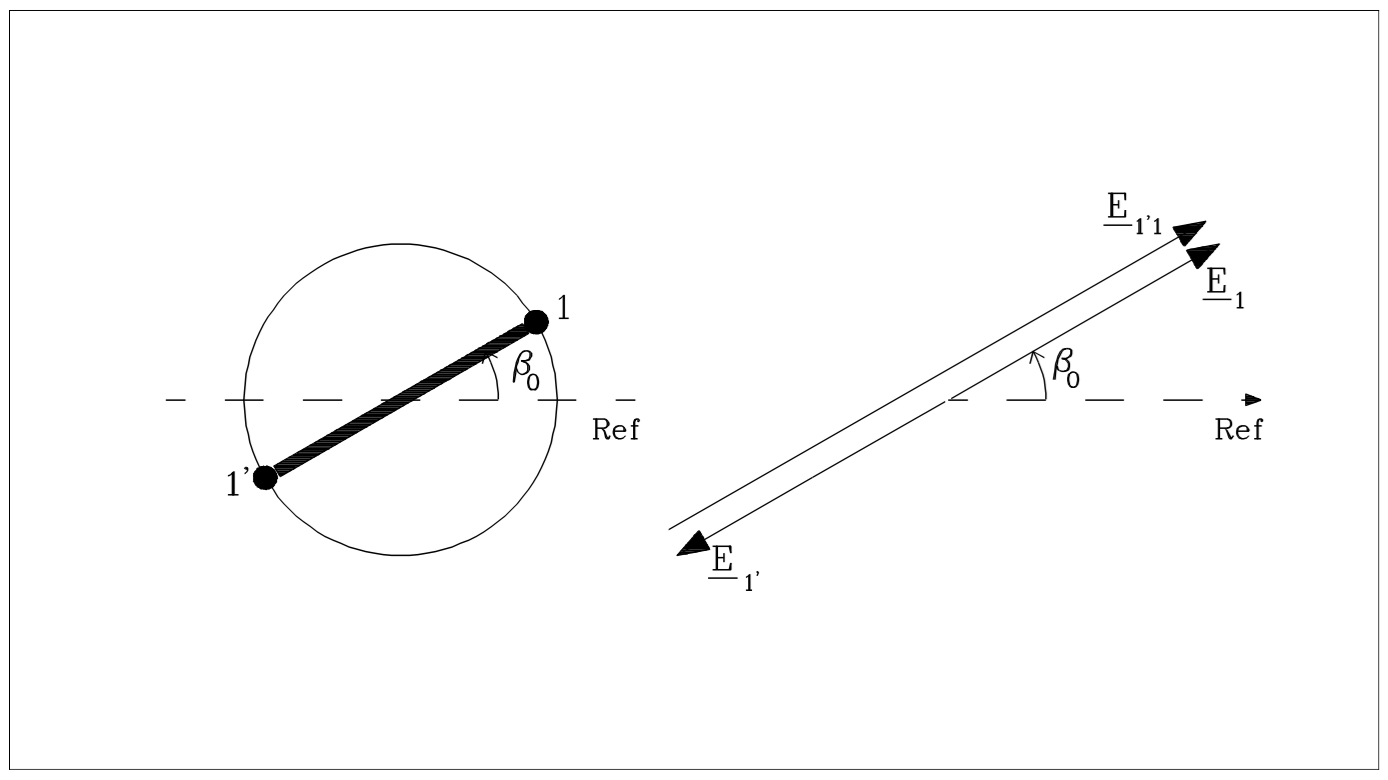
\includegraphics[scale=0.2]{ch2/image3} 
			\captionof{figure}{}
			\end{wrapfigure}
		Si la répartition spatiale de l'induction est sinusoïdale, la répartition temporelle de la f.e.m l'est aussi. En effet, si $B(\beta )= B^M\cos \beta$, on a d'après \autoref{eq:2.10} et $\beta _1 = \Omega _r t + \beta _0$
			\begin{equation}
			\begin{aligned}
				e_1 &= Blv = B^M lR\Omega _r \cos (\Omega _r t + \beta _1)\\
				 &= E_M \cos (\Omega _r t + \beta _1) \\
				 &= E\sqrt{2}\cos (\Omega _r t + \beta _1)
				\end{aligned}
			\end{equation}
		En phaseur, on l'exprime 
		\begin{equation}
			\underline{E_1} = E\sqrt{2} \angle \beta _0 = E\sqrt{2} e^{j\beta _0}
		\end{equation}
		Le conducteur de retour d'une spire diamétrale est décalé de $\pi$		
		\begin{equation}
			\underline{E_{1'}} = E\angle \beta _0 -\pi = -\underline{E_1}\qquad \Rightarrow \underline{E_{11'}} = 2\underline{E_1}
		\end{equation}
		
		\subsubsection{Spire non diamétrale}
			\begin{wrapfigure}[6]{r}{5cm}
			\vspace{-5mm}
			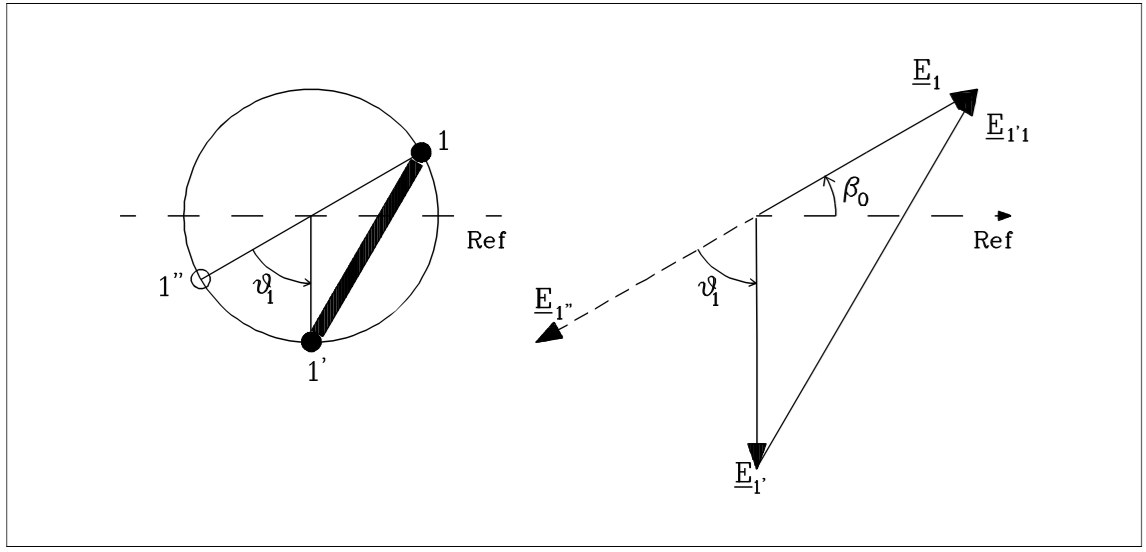
\includegraphics[scale=0.25]{ch2/image4} 
			\captionof{figure}{}
			\end{wrapfigure}
			Si 1' est décalé de $\theta_1$ par rapport à 1'' d'une spire 
			diamétrale, la connexion d'extrémité est plus courte (bien) 
			mais la tension à ses bornes est plus faible (bof).\\\\
		
		\subsubsection{Enroulement}
		\begin{wrapfigure}[9]{l}{6.5cm}
			\vspace{-5mm}
			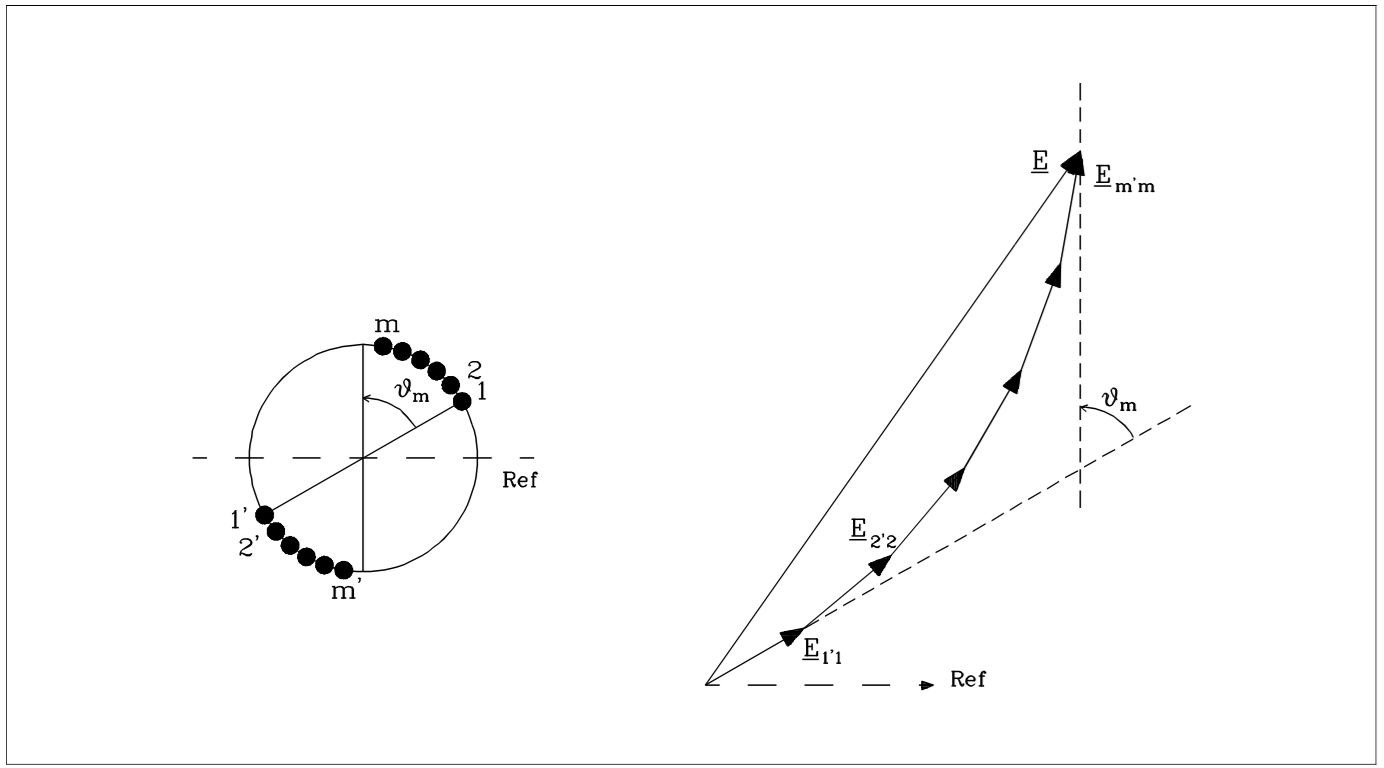
\includegraphics[scale=0.25]{ch2/image5} 
			\captionof{figure}{}
			\end{wrapfigure}
		D'un point de vue économique, il est préférable de considérer 
		plusieurs spires. Soit 22', une spire décalée de $\theta_1$ 
		par rapport à 11' ; le phaseur à ses bornes est lui aussi 
		déphasé de $\theta_1$ :
		\begin{equation}
		\underline{E_{2'2}} = \underline{E_{1'1}}e^{j\theta_1}
		\end{equation}
		\textbf{Attention !} On peut mettre ces deux spires en série, 
		mais pas en parallèle\footnote{Pq ?}.\\
		
		On peut ajouter $m$ spires sur un arc $\theta_m$ du rotor. 
		Néanmoins, 	il n'est pas économique de dépasser $\theta_m = 
		\pi/3$, l'accroissement de tension étant faible. Pour $\theta_m = 
		\pi/3$, le rotor peut accueillir trois enroulements indépendants 
		aux bornes desquels on peut obtenir une f.e.m. d'amplitudes 
		égale, mais décalée de $2\pi/3$ : c'est le système \textbf{triphasé 
		équilibré}. Une telle machine a la particularité de posséder l'induit sur 
		le stator. Il s'agit d'une machine synchrone à rotor lisse à 
		une paire de pôles (non-étudié ici).\\
		
		Au premier chapitre, nous avons vu comment connecter les enroulements 
		pour garantir une distribution économique de l'énergie. Si des 
		impédances égales sont branchées sur les enroulements, le système 
		est triphasé équilibré : un moteur synchrone connecté à ce réseau 
		entraînera une vitesse constante.
		
		
		\subsubsection{Machine à courant continu}
		Les extrémités de la spire sont connectées à un secteur conducteur 
		tournant, isolé du précédent. Sur ces secteurs appelés \textit{lames 
		de collecteur} reposent deux balais fixes diamétralement opposés. La 
		commutation est le passage d'un balai d'un secteur à un autre. En bref, 
		si un conducteur en forme de spire, parcouru par un courant, est placé
		dans un champ magnétique, il est soumis à des forces de Laplace. Ces forces 
		créent un couple de rotation qui fait tourner la spire sur son axe. Quand 
		la spire a fait un demi tour, il faut inverser la polarité pour inverser le 
		sens des forces et continuer le mouvement. ce sera le rôle du collecteur.
		
		\subsubsection{Machine à plusieurs paire de pôles}
		Simple généralisation : la période d'induction n'est plus de $2\pi$ mais 
		de $2\pi/p$. Pour en tenir compte on définit des angles électriques multiples des mécaniques
		\begin{equation}
			\beta _{él} = p\beta _{méca} \qquad \omega = \Omega _{r,él} = p\Omega _{r,méca}
		\end{equation}
		
		
		
\section{Composants des machines électriques}
Pour canaliser le champ magnétique on utilise du fer : on forme un circuit 
magnétique. Le circuit électrique est généralement en cuivre. Pour séparer les composants, un isolant 
est utilisé. Comme ça chauffe, il sera nécessaire de refroidir toute machine 
électrique.

	\subsection{Circuit magnétique}
	Son rôle est de conduire le flux qui devra agir sur les courants circulant 
	dans le circuit électrique placé au milieu de l'entrefer. Ce circuit est 
	constitué d'un solide de forte perméabilité magnétique imposant\footnote{Une 
	partie parvient tout de même à s'échapper : le flux de dispersion magnétique.} 
	le trajet des lignes de champs d'où le nom \textit{circuit magnétique} par analogie 
	à l'\textit{électrique}.
	
	\subsubsection{Dispersion magnétique}
	Si le fer possède une perméabilité $\mu _{fer}$ de l'ordre de 1000 fois plus grand que l'air, il y a quand même un flux qui passe en dehors du fer : c'est le \textbf{flux de dispersion}. Considérons un circuit magnétique entouré d'un circuit électrique (inducteur). On a 
	\begin{equation}
		\Phi _{tot} = \Phi _{magné} + \Phi _{dispers} = v \Phi _{magné} \qquad avec \qquad v = 1+\frac{\Phi_{dispers}}{\Phi _{magné}}
	\end{equation}
	$v$ est le \textbf{coefficient de Hopkinson}.
	
	\subsubsection{Pertes dans le fer}
	Le fer actif des machines est soumis à un cycle d'inversion d'aimantation périodique soit parce que le flux a une amplitude constante mais que la position varie soit inversement. \\
	
	\textsc{Pertes hystérétiques}\\
	\begin{wrapfigure}[8]{l}{4cm}
	\vspace{-5mm}
	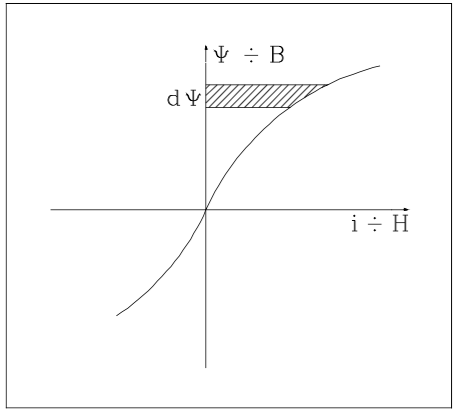
\includegraphics[scale=0.4]{ch2/image6} 
	\captionof{figure}{}
	\label{fig:2.6}
	\end{wrapfigure}
	L'énergie absorbée par le circuit est
	\begin{equation}
		dW = Pdt = vidt = id\psi
	\end{equation}
	Sur la \autoref{fig:2.6} on peut voir cette expression par l'air hachuré pour $\Delta \psi$. Si la relation entre $\psi$ et i est biunivoque, l'énergie sera tantôt absorbée tantôt redistribué tel que l'intégrale est nulle après une période. Par contre, si ce n'est pas le cas, l'énergie absorbée en une période est proportionnelle à l'air du cycle d'hystérèse B-H. Pour réduire cette perte, on cherchera le matériau d'hystérèse la plus étroite. \\
	
	\textsc{Pertes par courant de Foucault}\\
	\begin{wrapfigure}[18]{r}{2.5cm}
	\vspace{-5mm}
	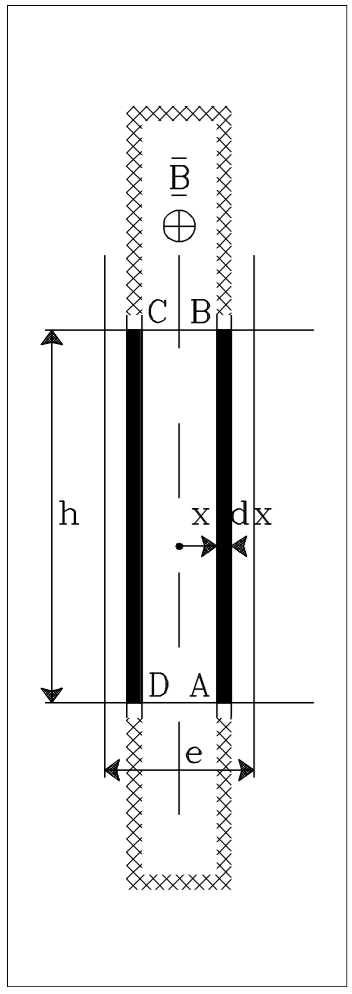
\includegraphics[scale=0.4]{ch2/image7} 
	\captionof{figure}{}
	\label{fig:2.7}
	\end{wrapfigure}
	Considérons une tôle d'épaisseur $e$ et prenons un élément de surface ABCD au sein de celui-ci, de hauteur $h$, longueur $l$ et constitué d'un tube d'épaisseur $dx$. La f.e.m induite sera d'après la loi de Faraday $e = \int \vec{E}\, \vec{dl} = -\int \frac{\D \vec{B}}{\D  t} \vec{dS}$
	\begin{equation}
		\sqrt{2} E_{ABCD} = 2\pi f B_M 2xh
	\end{equation}	 
	La résistance du circuit et par Ohm, le courant sont 
	\begin{equation}
		R = \rho\frac{2h}{ldx} \qquad et \qquad dI = \frac{\sqrt{2}\pi f B_M lxdx}{\rho}
	\end{equation}
	La perte de puissance vaut alors
	\begin{equation}
		dP_{pF} = EdI = \frac{(\sqrt{2}\pi f B_M)^2  2lhx^2dx}{\rho}
	\end{equation}
	Après intégration de la puissance de 0 à $e/2$	et sachant que\footnote{Démontré plus tard dans le cours.} $V = \sqrt{2}\pi f NB_MS$, on a 
	\begin{equation}
		P_{pF} = \mbox{volume}\frac{V^2e^2}{12\rho N^2 S^2}
	\end{equation}
	où $S$ est supposé constant et $V$ est la valeur efficace de la tension au borne d'un circuit sans résistance. On conclue que les pertes par Foucault sont proportionnelles au carré de la fréquence alors que les pertes par hystérèse sont directement proportionnelle à la fréquence. \\
	En pratique on réalise de tels circuits par empilage de tôles de petites épaisseur ($e^2$ dans l'équation) et les pertes globales sont de l'ordre de $3.5\, W/kg$. \footnote{Ramené à $1\, W/kg$ avec du silicium.}
	
	\subsubsection{Matériau utilisé}
	\begin{wrapfigure}[6]{r}{5cm}
	\vspace{-5mm}
	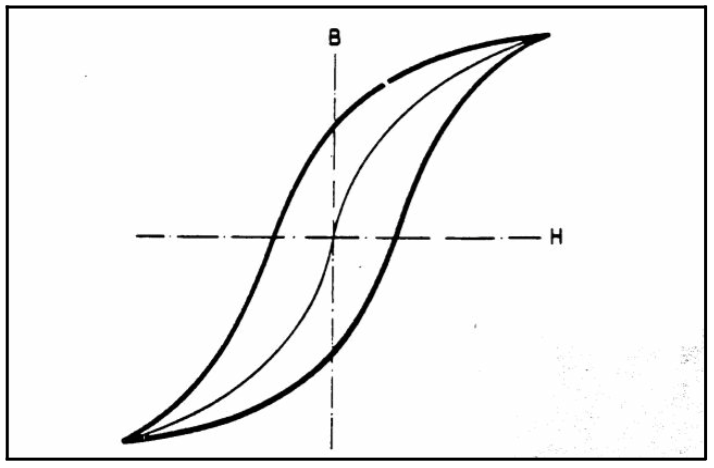
\includegraphics[scale=0.4]{ch2/image8} 
	\captionof{figure}{}
	\label{fig:2.7}
	\end{wrapfigure}
	L'acier, la fonte, le fer, \dots Le plus important est la loi qui lie l'induction au champ magnétique. Ce n'est 
	pas quelque chose de linéaire : la perméabilité $\mu _r$ d'un matériau varie en 
	fonction du champ qui lui est appliqué. Pour représenter ça, on regarde 
	les \textit{courbes de magnétisation.} On y observe le phénomène de saturation. 
	
	\subsection{Circuit électrique}
	\textsc{Rappel.} L'\textbf{inducteur} est chargé de créer le flux utile et l'
	\textbf{induit} chargé de créer les f.e.m (génératrices) ou couples (moteurs).\footnote{Wiki : L'inducteur est un organe 
	électrotechnique, généralement un électroaimant, ayant comme fonction d'induire 
	un champ électromagnétique dans un induit servant à chauffer toutes sortes de 
	conducteurs comme des métaux de toutes sortes.}
	
		\subsubsection{Disposition des enroulements}
		\textsc{Inducteur}\\
		Il peut être situé au rotor. On utilise des aimants permanents pour les 
		petites puissances. On distingue les inducteurs à pôles saillants (enroulement autour d'aimant) et ceux à pôles lisse (conducteurs déposés dans les encoches).\\
		
		\textsc{Induit}\\
		Les conducteurs sont généralement isolés entre eux. On utilise souvent 
		un bobinage creux pour le refroidissement, déposé dans une encoche fermée par des cales (meilleurs résistance mécanique et réduction de l'entrefer).  
		
		\subsubsection{Groupement des conducteurs}
		L'association des conducteurs d'une machine est le \textbf{bobinage}. 
		\begin{description}
		\item[Conducteurs.] On peut utiliser un conducteur (massif ou creux) ou plusieurs conducteur en parallèle pour 
		véhiculer un courant $I$ de densité allant de $2.5$ à $5\, A/mm^2$.
		\item[Spire.] Constituée de deux conducteurs avec les tensions déphasées de 180\degres .
		\item[Bobine.] Lorsqu'il y a plusieurs conducteurs par encoche.
		\item[Phase.] Un groupe de bobines associées en série ou en parallèle.
		\end{description}
		
	\subsubsection{Pertes joules dans les conducteurs}
	\begin{wrapfigure}[10]{l}{3cm}
	\vspace{-5mm}
	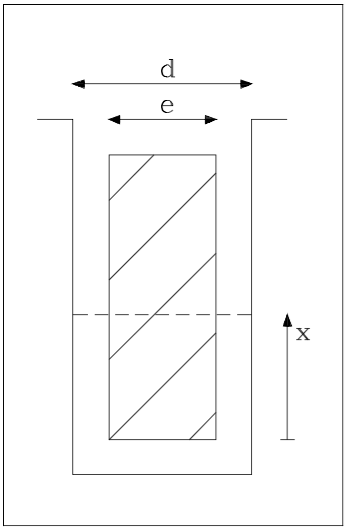
\includegraphics[scale=0.4]{ch2/image9} 
	\captionof{figure}{}
	\label{fig:2.9}
	\end{wrapfigure}
	Étudions la densité de courant dans un conducteur d'encoche. Les courants 
	circulants engendrent des pertes ($P_J = RI^2$ où $R=\rho l/S$ en continu).
	Si le conducteur est massif, en continu, la densité de courant $J=I/S$ est 
	constante. Démontrons par l'absurde que ce n'est pas le cas en alternatif.\\
	
	Soit un conducteur massif dans une encoche et supposons $J = \text{cste}$ :
	\begin{equation}
	\begin{array}{lll}
	
	& H(x)d + 0 &= \displaystyle\int_0^x Jedx\\
	\Leftrightarrow& H(x) &= \dfrac{Je}{d}x
	\end{array}
	\end{equation}
	où $H$ varie linéairement avec $x$. Le flux embrassé par le circuit constitué 
	par cette partie du conducteur et le retour à l’infini vaut, par unité de 
	longueur :
	\begin{equation}
	\begin{array}{ll}
	\dfrac{\Delta \phi(x)}{\Delta l} &= \text{ cste } - \int_0^x B(x)dx\\
 	&= \text{ cste } - \mu_0\int_0^x H(x) dx\\
	&= \text{ cste } - \dfrac{\mu_0Je}{d}\dfrac{x^2}{2}
	\end{array}
	\end{equation}
	La chute de tension inductive par unité de longueur du conducteur dépend de 
	la position du filet de courant (et de la fréquence) : il n'est pas correct 
	de supposer $J = \text{cste}$ : la densité de flux est plus importante à la 
	"surface".\\
	La fréquence augmente également les pertes (résistance plus importante). On 
	peut utiliser des barres de Roebel obligeant le courant à passer à la surface 
	et en profondeur de l'encoche pour contrer au maximum cet effet.
	
	\subsubsection{Matériau utilisé}
	Les matériaux les plus utilisés sont le cuivre et l'alluminium. Considérons deux conducteur de sections différentes mais de résistance et longueur égale. On a
	\begin{equation}
		\rho _{Al}\frac{l}{S_{Al}} = \rho _{Cu}\frac{l}{S_{Cu}} \qquad \Rightarrow S_{Al} = 1.6 \, S_{Cu}
	\end{equation}
	On voit donc que la surface d'Al est plus grande que celle du Cu, mais la masse volumique de l'Al étant inférieur à celle de Cu, l'Al est plus avantageux\footnote{Mais encombrements et résistance mécanique moindre dans les machines.}. 
	
	\subsection{Isolation des machines}
		\subsubsection{Loi de Montsinger - Vieillissement des isolants}
		La température déteriore la qualité de l'isolant. Une loi expérimentale 
		décrit cet effet
		\begin{equation}
		t = ab^{-\theta}
		\end{equation}
		où $t$ est la durée de vie, $a,b$ des constantes pour un isolant donné 
		et $\theta$ la température. On peut l'écrire :
		\begin{equation}
		\log t = \log a - \theta\log b
		\end{equation}
		où $\log t$ est une fonction linéaire de $\theta$. Ainsi, élever la 
		température de 6 à 10$^\circ$ réduit la durée de vie de moitié !
		
	\subsection{Refroidissement}
		\subsubsection{Agents de refroidissement}
		Le plus courant est d'utiliser l'air, un ventilateur. Des ventilations 
		intérieures ou extérieures (enceinte close) pour une atmosphère fort 
		polluée existent également. L'hydrogène (conductibilité thermique >>) peut également refroidir en 
		le faisant circuler dans les conducteurs. Les diélectriques liquides 
		sont également une option.
		
\section{Grandeurs caractéristiques des machines électriques}
	\subsection{Grandeurs nominales}
	Une grandeur physique est dite \textit{nominale} lorsque l'appareil peut 
	fonctionner indéfiniment à celle-ci sans subir d'usure (avec un coefficient 
	de sécurité).\\
	La \textit{puissance nominale} est plus subtile, il faut savoir de quoi on 
	parle :
	\begin{itemize}
	\item[$\bullet$] Pour une génératrice à courant continu, c'est la puissance électrique développable (en kW) à ses 
	bornes
	\item[$\bullet$] Pour un alternateur, c'est la puissance électrique 
	apparente développable (en kVA)
	\item[$\bullet$] Pour un moteur, il s'agit de la puissance mécanique 
	disponible (en kW)
	\end{itemize}
	
	\subsection{Rendements des machines}
	Par définition, on défini le rendement 
	\begin{equation}
	\eta = \frac{P_u}{P_a}
	\end{equation}
	où $P_u$ est la puissance utile à la sortie et $P_a$ la puissance 
	absorbée. On peut écrire cette formule
	\begin{equation}
	\eta = \frac{P_u}{P_a} = \frac{P_a-p}{P_a} = \frac{P_u}{P_u+p}
	\end{equation}
	où $p$ est la perte. Celles-ci ont un terme fixe et un terme variable avec 
	la puissance apparente $S$. On utilisera la dernière égalité, plus précise\footnote{
	Pour les machines génératrices, $P_a$ est mécanique et $P_u$ électrique. C'est 
	l'inverse pour une machine motrice}. Les pertes peuvent être mécaniques, 
	due aux fer, \dots\\
	
	Pour le cuivre, les pertes sont variable en fonction de $I$ : $P_{p,Cu} = 3
	RI^2$. Comme la tension est supposée constante : $P_{p,Cu} = kV^2I^2 = kS^2$. 
	Les pertes totales s'expriment ainsi de la forme $p = a+bS^2$ et, par exemple, 
	on peut écrire l'expression du rendement :\footnote{La puissance absorbée correspond à la puissance active.}
	\begin{equation}
	\eta = \frac{P_a-p}{P_a} = \dfrac{S\cos\varphi-a-bS^2}{S\cos\varphi}
	\end{equation}
	Dans le cas où $\cos \varphi$ est constant, la valeur maximale du rendement est donnée par
	\begin{equation}
	\frac{d\eta}{dS} = 0\qquad \Leftrightarrow\qquad S = \sqrt{\frac{a}{b}}
	\end{equation}
	pour lequel, les pertes constantes sont égales aux pertes variables. \\
	Pour le cas de $\cos \varphi$ variable, on doit tracer des courbes de rendement. 
	La forme de la courbe rendement souhaitée dépend des conditions d'utilisation.\\
	Pour mesurer le rendement, il est plus intéressant de mesurer les pertes que 
	de mesurer la puissance électrique et mécanique. On peut le faire en mesurant 
	l'échauffement ou en mesurant chaque perte une à une, par essai.
	
	
	\subsection{Caractéristiques des machines tournantes}
		\subsubsection{Moteurs}
			La caractéristique fondamentale d'un moteur est la relation entre le couple moteur et la vitesse de rotation. Pareillement pour la charge, on définit le couple résistance 
			\begin{equation}
				C_m = f(N) \qquad C_r = f(N)
			\end{equation}
			Le fonctionnement de l'ensemble moteur + charge est fixé par la position relative des deux caractéristiques. \\
			
			\textsc{Mise en vitesse}\\
				Les phénomènes transitoire mécanique ont des constantes de temps plus élevées que les phénomènes électriques (établissement de flux). De ce fait, on suppose le régime électrique établi. Pour que la machine démarre, il faut que $C_{md} > C_{r0}$\footnote{Couple moteur de démarrage plus grand que couple résistance initial.}. De plus, il ne faut pas que l'écart entre les deux grandeurs soit trop grand pour éviter une trop grande accélération. On définit le \textbf{couple accélérateur}
				\begin{equation}
					C_m - C_r = J\frac{d\Omega _r}{dt}
				\end{equation}
	où $J$ est le moment d'inertie. Il faut que le temps de démarrage soit court, mais d'autre part il faut éviter l'échauffement. Pour la durée, reprenons l'équation et intégrons membre à membre
	\begin{equation}
		\int _0^{\Omega _n} \frac{d\Omega _r}{C_m	- C_r} = \frac{1}{J}\int _0 ^{t_d} dt = \frac{t_d}{J}
	\end{equation}
	Par difficulté d'exprimer les couples, on procède à des intégrations numériques.\\
	
	\textsc{Vitesse normale}\\
	La vitesse de régime est atteinte lorsque $\frac{d\Omega _r}{dt} = 0$ donc quand les deux couples sont égaux\footnote{Les vitesses de rotation ne sont égaux que dans le cas d'accouplement direct.}. Il faut dès lors que l'équilibre soit stable. Si ce n'est pas le cas, soit on a un emballement du moteur, soit la machine cale et s'arrête progressivement (dans le cas d'un couple résistant pour lequel les courbes caractéristiques ne se croisent pas). \\
	
	\textsc{Génératrice}\\
	C'est la caractéristique externe qui nous intéresse dans ce cas, pour $\cos \varphi\text{ et }N = cst$ on a $U_g = f(I)$ et $U_r = f(I)$ (circuit de consommation). Le point de fonctionnement $U_g = U_r$, $I_g = I_r$ sera stable si le système revient à son état initial quand on fait varier $I$. 
		
		
		
		
		
		
		
		
		
		
		
		
		
		
